\documentclass{article}

\usepackage[left=2cm,right=2cm, top=2cm, bottom = 2cm]{geometry}
\usepackage{amsfonts}
%%%\usepackage{array}

\usepackage{amsmath}
\usepackage{xcolor}

\usepackage{tikz}
\usepackage{subfigure}

\pagestyle{empty}

\setlength{\tabcolsep}{15pt}
%%%\renewcommand{\arraystretch}{2.5}

%%%\makeatletter
%%%\newcommand{\thickhline}{%
%%%    \noalign {\ifnum 0=`}\fi \hrule height 2pt
%%%    \futurelet \reserved@a \@xhline
%%%}
%%%\newcolumntype{!}{@{\hskip\tabcolsep\vrule width 2pt\hskip\tabcolsep}}
%%%\makeatother

\newcommand{\deriv}[3][]{\frac{\mathrm{d}^{#1} #2}{\mathrm{d}#3^{#1}}}




\begin{document}


\Large






Cautionary example: Let $f(t)=e^{-t}\sin(2\pi t)$. This sort of function occurs in practice as the position of a mass on a spring, with the exponential decay coming from friction or other resistive forces. Clearly $f(t)=0$ precisely when $\sin(2\pi t)=0$, so the roots of $f$ are $\frac{n}{2}$ for all integer values of $n$. Starting with $t_0=0.25$, perform the Newton-Raphson method. Can you explain what is happening?

% f'(t) = e^{-t}(2\pi \cos(2\pi t)-\sin(2\pi t)). f'(1/4) = e^{-0.25}(2\pi\cos(\pi/2) - \sin(\pi/2)) = -e^{-0.25}
% f(0.25) = e^{-0.25}

\begin{center}
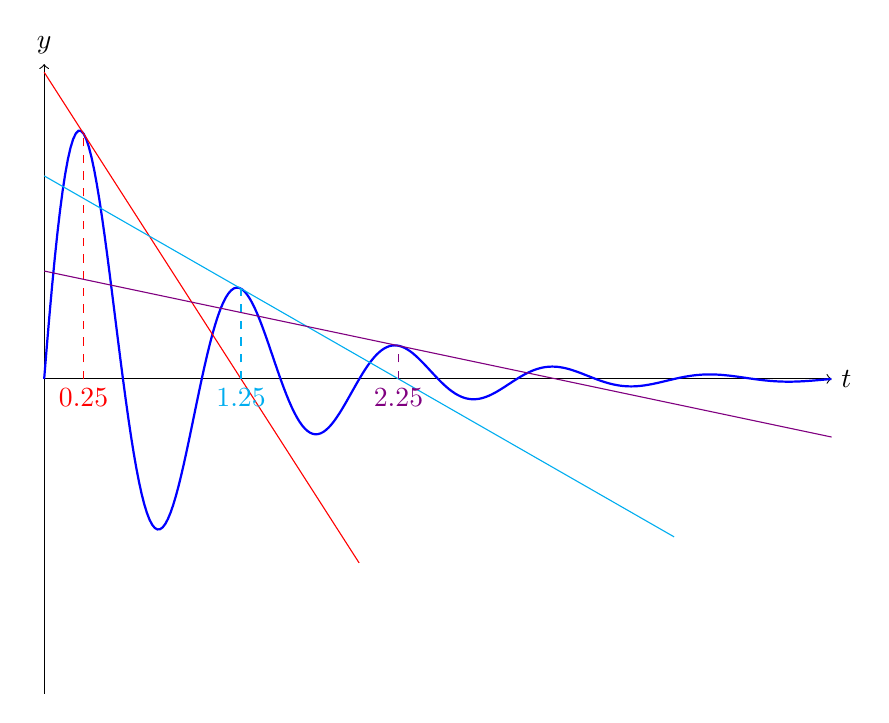
\begin{tikzpicture}
	\draw[->] (0,0) -- (10,0);
	\node[right] at (10,0) {$t$};
	\draw[->] (0,-4) -- (0,4);
	\node[above] at (0,4) {$y$};
	
	\draw[thick,blue,domain=0:10,samples=300] plot (\x,{4*exp(-0.5*\x)*sin(3.14*\x r)});
	
	\draw[red,domain=0:4] plot (\x, {4*(-exp(-0.25)*(0.5*\x-0.25) + exp(-0.25))});
	\draw[red,dashed] (0.5,0) -- (0.5,3.115);
	\node[red,below] at (0.5,0) {$0.25$};
	
	\draw[cyan,dashed] (2.5,0) -- (2.5,1.146);
	\node[cyan,below] at (2.5,0) {$1.25$};
	\draw[cyan,domain=0:8] plot (\x, {4*( -exp(-1.25)*(0.5*\x - 1.25) + exp(-1.25)) )});
	
	\draw[violet,dashed] (4.5,0) -- (4.5,0.4216);
	\node[violet,below] at (4.5,0) {$2.25$};
	\draw[violet,domain=0:10] plot (\x, {4*( -exp(-2.25)*(0.5*\x - 2.25) + exp(-2.25) )});
\end{tikzpicture}
\end{center}

\begin{align*}
	t_{n+1}&=t_n-\frac{f(t_n)}{f'(t_n)}\\
	&= t_n - \frac{e^{-t_n}\sin(2\pi t_n)}{e^{-t_n}(2\pi\cos(2\pi t_n)-\sin(2\pi t_n))}\\
	&=t_n -\frac{\sin(2\pi t_n)}{2\pi\cos(2\pi t_n)-\sin(2\pi t_n)}.
\end{align*}

If $t_n=n+\frac{1}{4}$, then

\begin{align*}
	t_{n+1}&= n+\frac{1}{4} - \frac{\sin\left(2\pi n + \frac{\pi}{2}\right)}{2\pi\cos\left(2\pi n + \frac{\pi}{2}\right)-\sin\left(2\pi n+\frac{\pi}{2}\right)}\\
	&= n+\frac{1}{4} - \frac{\sin\left(\frac{\pi}{2}\right)}{2\pi\cos\left(\frac{\pi}{2}\right)-\sin\left(\frac{\pi}{2}\right)}\\
	&= n+\frac{1}{4} - \frac{1}{0-1}\\
	&= (n+1) + \frac{1}{4}.
\end{align*}

So if we start at $t_0=0.25$, then we get $t_n=n+0.25$ for each $n$, and we never converge to a root! However, if we change our starting point very slightly, the problem disappears. Starting at $t_0=0.24$, we converge to the root at 2 in 4 iterations, whereas if we start at $t_0=0.26$, we converge to the root at 1 in 3 iterations.





\end{document}